\section{Rancangan Solusi}
\label{sec:rancangan-solusi}

Dibangun sebuah rancangan solusi berupa skenario pengujian yang dilakukan dalam penelitian tugas akhir, yang dapat dilihat pada Gambar \ref{fig:rancangan-solusi}. Berdasarkan Gambar \ref{fig:rancangan-solusi}, tidak ditambahkan \textit{dataset} baru, melainkan menggunakan \textit{dataset} yang sudah disediakan pada IndoLEM. Teknik PEFT yang digunakan adalah LoRA (\textit{Low-Rank Adaptation}), \textit{Prefix-Tuning}, dan \textit{Bottleneck Adapter}. Hasil pengujian berupa kinerja dari teknik PEFT serta penggunaan sumber daya dari setiap eksperimen.

\begin{figure}[ht]
    \centering
    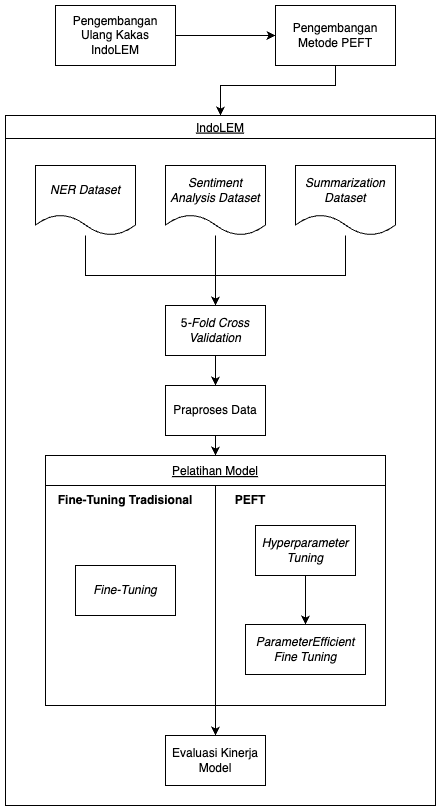
\includegraphics[height=0.6\textheight]{chapter-3/rancangan_solusi.png}
    \caption{Rancangan Solusi}
    \label{fig:rancangan-solusi}
\end{figure}

Sebelum bisa dilakukan pelatihan dan evaluasi model, diperlukan adanya pengembangan ulang pada kakas IndoLEM serta metode PEFT. Pengembangan ulang ini dilakukan agar pengembangan metode PEFT bisa dilakukan. Pengembangan ulang kakas IndoLEM  menggunakan beberapa pustaka, salah satunya adalah Transformers dan Torch. Pustaka Transformers diperlukan untuk melakukan pemuatan model, praproses data, dan penggunaan Trainer untuk standardisasi. Lalu, pustaka Torch digunakan untuk menggunakan CUDA yang memanfaatkan GPU untuk melatih model. Selain itu, pustaka Wandb dan Huggingface juga  dipakai untuk melakukan sinkronisasi pada \textit{cloud}. Dengan sinkronisasi ini, hasil pelatihan model dan hasil evaluasi dapat dilihat pada situsnya yang  memudahkan proses eksperimen. 

Pengembangan metode PEFT pada kakas IndoLEM  menggunakan pustaka Adapters. Model yang dimuat oleh pustaka Transformers perlu diinisiasi oleh pustaka Adapters untuk dapat berjalan menggunakan metode PEFT. Untuk dapat menjalankan proses pelatihan dengan metode PEFT, perlu digunakan Trainer yang berasal dari pustaka Adapters, yaitu AdapterTrainer yang  melakukan \textit{freeze} pada parameter model dan  menggunakan parameter yang sesuai dengan metode PEFT-nya tersebut.

Sesuai dengan banyaknya tugas evaluasi yang diimplementasikan, harus disesuaikan dengan banyaknya tugas evaluasi tersebut, yaitu \nlptask. Setiap \textit{dataset}  dilakukan 5-\textit{fold cross validation} yang membagi setiap \textit{dataset} menjadi 5 bagian \textit{dataset} validasi yang berbeda. Metode \textit{cross validation} ini sudah dilakukan pada kakas IndoLEM, sehingga \textit{dataset} sudah terbagi menjadi 5-\textit{fold}. Untuk setiap \textit{fold}-nya, \textit{dataset}  dilakukan praproses data, pelatihan model, dan evaluasi kinerja. Praproses data ini dilakukan dengan melakukan \textit{padding}, tokenisasi, dan juga mengatur \textit{mapping} dengan labelnya. 

Proses pelatihan model dibagi menjadi dua, yaitu dengan menggunakan \textit{fine-tuning} dan menggunakan metode PEFT. Pelatihan model  dilakukan pada lingkungan pelatihan yang sesuai yaitu pada lingkungkan \textit{cloud} yang menggunakan GPU khusus untuk pelatihan model. Pelatihan dengan \textit{fine-tuning} mengikuti \textit{hyperparameter} pada penelitian terkaitnya. Sedangkan, untuk metode PEFT  dilakukan \textit{hyperparameter tuning} untuk metode PEFT-nya.

Selanjutnya, untuk setiap hasil pelatihan model, dilakukan evaluasi dengan menggunakan \textit{dataset} validasi-nya. Metrik evaluasi yang digunakan tergantung pada tugas evaluasinya. Tugas evaluasi \textit{classification} (NER dan \textit{sentiment analysis})  menggunakan \textit{accuracy} dan F1 \textit{score}. Sedangkan, tugas evaluasi \textit{generation} (\textit{summarization})  menggunakan ROUGE \textit{score}.

